\documentclass[10.5pt]{article}
\usepackage{amsmath,amssymb,amsthm}
\usepackage{listings}
\usepackage{graphicx}
\usepackage[shortlabels]{enumitem}
\usepackage{tikz}
\usepackage[margin=1in]{geometry}
\usepackage{fancyhdr}
\usepackage{epsfig} %% for loading postscript figures
\usepackage{amsmath}
\usepackage{float}
\usepackage{amssymb}
\usepackage{caption}
\usepackage{subfigure}
\usepackage{graphics}
\usepackage{titlesec}
\usepackage{mathrsfs}
\usepackage{amsfonts}
\usepackage{indentfirst}
\usepackage{fancybox}
\usepackage{tikz}
\usepackage{algorithm}
\usepackage{algcompatible}

% my new command

\newcommand{\liminfty}{\lim_{n\to\infty}}

\renewcommand{\baselinestretch}{1.2}%Adjust Line Spacing
%\geometry{left=2.0cm,right=2.0cm,top=2.0cm,bottom=2.0cm}% Adjust Margins of the File
\usepackage{tikz-qtree}
\usetikzlibrary{graphs}
\tikzset{every tree node/.style={minimum width=2em,draw,circle},
	blank/.style={draw=none},
	edge from parent/.style=
	{draw,edge from parent path={(\tikzparentnode) -- (\tikzchildnode)}},
	level distance=1.2cm}
\setlength{\parindent}{0pt}
%\setlength{\parskip}{5pt plus 1pt}
\setlength{\headheight}{13.6pt}
\newcommand\question[2]{\vspace{.25in}\hrule\textbf{#1: #2}\vspace{.5em}
\hrule\vspace{.10in}}
\renewcommand\part[1]{\vspace{.10in}\textbf{(#1)}}
\pagestyle{fancyplain}
% Create horizontal rule command with an argument of height
\newcommand{\horrule}[1]{\rule{\linewidth}{#1}}
% Set the title here
\title{
	\normalfont \normalsize
	\textsc{ShanghaiTech University} \\ [25pt]
	\horrule{0.5pt} \\[0.4cm] % Thin top horizontal rule
	\huge CS101 Algorithms and Data Structures\\ % The assignment title
	\LARGE Fall 2021\\
	\LARGE Homework 1\\
	\horrule{2pt} \\[0.5cm] % Thick bottom horizontal rule
}
% wrong usage of \author, never mind
\author{}
\date{Due date: 23:59, September 26, 2021}

\newtheorem{Q}{Question}
% set the header and footer
\pagestyle{fancy}
\lhead{CS101 Algorithms and Data Structures}
\chead{Homework 1}
\rhead{Due date: 23:59, September 26, 2021}
\cfoot{\thepage}
\renewcommand{\headrulewidth}{0.4pt}

% special settings for the first page
\fancypagestyle{firstpage}
{
	\renewcommand{\headrulewidth}{0pt}
	\fancyhf{}
	\fancyfoot[C]{\thepage}
}

% Add the support for auto numbering
% use \problem{title} or \problem[number]{title} to add a new problem
% also \subproblem is supported, just use it like \subsection
\newcounter{ProblemCounter}
\newcounter{oldvalue}
\newcommand{\problem}[2][-1]{
	\setcounter{oldvalue}{\value{secnumdepth}}
	\setcounter{secnumdepth}{0}
	\ifnum#1>-1
	\setcounter{ProblemCounter}{0}
	\else
	\stepcounter{ProblemCounter}
	\fi
	\section{Problem \arabic{ProblemCounter}: #2}
	\setcounter{secnumdepth}{\value{oldvalue}}
}
\newcommand{\subproblem}[1]{
	\setcounter{oldvalue}{\value{section}}
	\setcounter{section}{\value{ProblemCounter}}
	\subsection{#1}
	\setcounter{section}{\value{oldvalue}}
}

\definecolor{blve}{rgb}{0.3372549 , 0.61176471, 0.83921569}
\definecolor{gr33n}{rgb}{0.29019608, 0.7372549 , 0.64705882}
\makeatletter
\lst@InstallKeywords k{class}{classstyle}\slshape{classstyle}{}ld
\makeatother
\lstset{language=C++,
	basicstyle=\ttfamily,
	keywordstyle=\color{blve}\ttfamily,
	stringstyle=\color{red}\ttfamily,
	commentstyle=\color{green}\ttfamily,
	morecomment=[l][\color{magenta}]{\#},
	classstyle = \bfseries\color{gr33n}, 
	tabsize=4
}

\begin{document}
	
	\maketitle
	\thispagestyle{firstpage}
	%\newpage
	\vspace{3ex}
	
	\begin{enumerate}
		\item Please write your solutions in English. 
		
		\item Submit your solutions to gradescope.com.  
		
		\item Set your FULL Name to your Chinese name and your STUDENT ID correctly in Account Settings. 
		
		\item If you want to submit a handwritten version, scan it clearly. Camscanner is recommended. 
		
		\item When submitting, match your solutions to the according problem numbers correctly. 
		
		\item No late submission will be accepted.
		
		\item Violations to any of the above may result in zero grade. 
	\end{enumerate}
	\newpage
	
  \question{1}{(5*2')Academic integrity}
    \begin{Q}
    Please determine who violated academic integrity (or committed plagiarism) in the following situations. A stands for Alice, B stands for Bob, N stands for None, AB stands for Both.
    \\ \\
    \textit{Note that you should write you answers of section 1 in the table below.}
\begin{table}[htbp]
	\begin{tabular}{|p{1.5cm}|p{1.5cm}|p{1.5cm}|p{1.5cm}|p{1.5cm}|}
		\hline 
		Q1 (a) & Q1 (b) & Q1 (c) & Q1 (d) & Q1 (e) \\ 
		\hline 
		 AB & N & AB & A & AB \\ 
		\hline 
	\end{tabular} 
\end{table}
    	\begin{enumerate}[(a)]
    		\item Alice and Bob are good friends, Alice asked if Bob could send her some code snippets so that she could have some ideas of what is going on in this homework (promising, of course, not copying his code). Bob agreed and sent his code repository to Alice, Alice copied the code and submitted to the CS 101 Platform.
    		
    		\item Bob is Alice's boyfriend. In order to enhance their romantic relationship, they studied together in the ShanghaiTech library and collaborated on an individual programming assignment. They discussed about the algorithm using the whiteboard but they didn't see any lines of code from each other.
    		    		
    		    		
    		\item Alice and Bob are roommates. Bob let Alice use his laptop to play APEX Legends, and Alice copied Bob's solution for a paper assignment.
    		
    		\item Alice found the solution for a specific assignment on github and copied it to her homework with some trivial modifications.
    		
    		\item Alice borrows Bob's computer to complete her programming assignment. Without looking at Bob's code, she accidentally submits her own assignment using Bob's account to the CS 101 Platform. After that, Alice and Bob resubmitted their assignments separately using their own accounts.
    		
    		\end{enumerate}
    \end{Q}
	
	\pagebreak

	
	%---------------------------------------------------------
\question{2}{(3*2') Multiple Choices}

Each question has one or more correct answer(s). Select all the correct answer(s). For each question, you get $0$ point if you select one or more wrong answers, but you get $1$ point if you select a non-empty subset of the correct answers.\\ \\
\textit{Note that you should write you answers of section 2 in the table below.}
\begin{table}[htbp]
	\begin{tabular}{|p{2cm}|p{2cm}|p{2cm}|p{2cm}|}
		\hline 
	Question 2 & Question 3 & Question 4  \\ 
		\hline 
	 A & D & A \\ 
		\hline 
	\end{tabular} 
\end{table}

\begin{Q}
	Using a single linked list to implement a stack, suppose you only keep the head of it, where should the pushes and pops be performed in the optimal way?
	\begin{enumerate}[(A)]
		\item Push in front of the first element, pop the first element
		\item Push in front of the first element, pop the last element
		\item Push after the first element, pop the first element
		\item Push after the last element, pop the last element
		\item Push after the last element, pop the first element
	\end{enumerate}
\end{Q}

\begin{Q}
 Suppose we use a circular array with index range from 0 to N - 1 to implement a queue, and currently Front is pointing at index $m$. We will know that if this queue is full the last element in it should be stored at index = \rule[-3pt]{1cm}{0.05em}. (Options below are mapped to \textbf{Integers Modulo N}: $\mathbb{Z}_N = \{0, 1, 2, ..., N-1\}$)
	\begin{enumerate}[(A)]
		\item $0$
		\item $m$
		\item $N-1$
		\item $m-1$
	\end{enumerate}
\end{Q}


\begin{Q}
	What function does the following code achieve?
	\rm{
\begin{lstlisting}[language=C++]
  void Q4(Queue &Q) 
  {
    Stack S;
	int d;
	S.InitStack();
	while(!Q.IsEmpty())
	{
	  d = Q.DeQueue();
	  S.Push(d);
	}
	while(!S.IsEmpty())
	{
	  d = S.Pop();
	  Q.EnQueue(d);
	}
  }
\end{lstlisting}
	}
	\begin{enumerate}[(A)]
		\item Use a stack to reverse a queue.
		\item Use a queue to reverse a stack.
		\item Use a stack to implement a queue.
		\item Use a queue to implement a stack.
	\end{enumerate}
\end{Q}

%-------------------------------------------------


\pagebreak

	\question{3}{(5'+5')Array for list}
	\begin{Q}
	In this question, we use two arrays: ``next" and ``value" to simulate a linked-list. 
	The elements at each index in ``next" and ``value" 
	are combined together to represent a node in the 
	linked-list, where ``next" represents the pointer 
	to the next node, and ``value" represents data in 
	the nodes.
	\begin{enumerate}[(a)]
		\item \textbf{(5')Linked list from array representation}
		

		Here are the two arrays of ``next" and ``value".
		Please draw the linked list presented by the two arrays.
		\begin{center}
		\begin{tabular}{|c|c|c|c|c|c|c|c|c|c|c|c|}
			\hline
			index&0&1&2&3&4&5&6&7&8&9\\
			\hline
			value&A&B&C&D&E&F&G&H&I&J\\
			\hline
			next&7&5&3&9&/&2&0&1&4&8\\
			\hline

		\end{tabular}
	\end{center}
	\begin{center}
		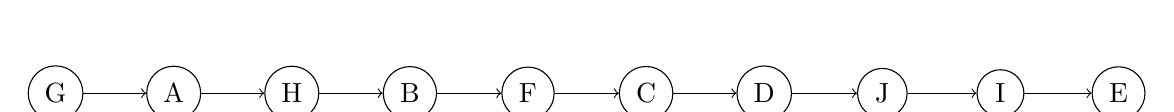
\begin{tikzpicture}
		%	\node[shape=circle,draw=black] (head) at (0,1.5) {Head};
			\node[shape=circle,draw=black] (G) at (0,0) {G};
			\node[shape=circle,draw=black] (A) at (1.5,0) {A};
			\node[shape=circle,draw=black] (H) at (3,0) {H};
			\node[shape=circle,draw=black] (B) at (4.5,0) {B};
			\node[shape=circle,draw=black] (F) at (6,0) {F};
			\node[shape=circle,draw=black] (C) at (7.5,0) {C};
			\node[shape=circle,draw=black] (D) at (9,0) {D};
			\node[shape=circle,draw=black] (J) at (10.5,0) {J};
			\node[shape=circle,draw=black] (I) at (12,0) {I};
			\node[shape=circle,draw=black] (E) at (13.5,0) {E};
		%	\node[shape=circle,draw=black] (nil) at (13.5,-1.5) {null};
		
		%	\path [->](head) edge node {} (G);
			\path [->](G) edge node {} (A);
			\path [->](A) edge node {} (H);
			\path [->](H) edge node {} (B);
			\path [->](B) edge node {} (F); 
			\path [->](F) edge node {} (C);
			\path [->](C) edge node {} (D);
			\path [->](D) edge node {} (J); 
			\path [->](J) edge node {} (I); 
			\path [->](I) edge node {} (E); 
		%	\path [->](E) edge node {} (nil); 



		\end{tikzpicture}
		\end{center}

		\vspace{3cm}
		\item \textbf{(5')Array representation for a linked list}
		 
		Fill in  the ``next" array in order to make the array and the linked-list showing below equivalent.

		\begin{center}
	
		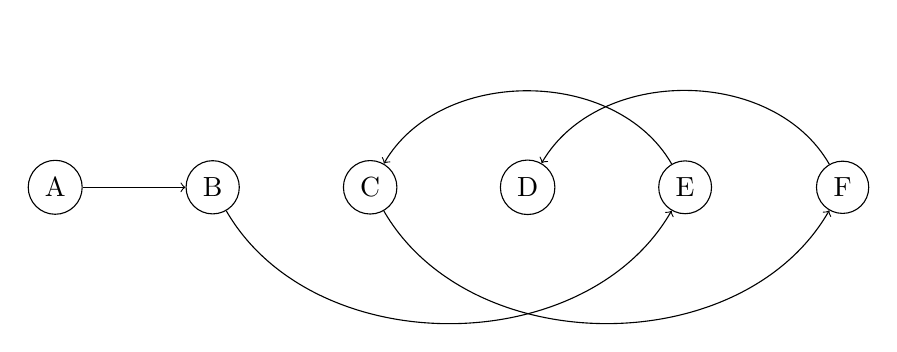
\begin{tikzpicture}
			\node[shape=circle,draw=black] (A) at (0,0) {A};
			\node[shape=circle,draw=black] (B) at (2,0) {B};
			\node[shape=circle,draw=black] (C) at (4,0) {C};
			\node[shape=circle,draw=black] (D) at (6,0) {D};
			\node[shape=circle,draw=black] (E) at (8,0) {E};
			\node[shape=circle,draw=black] (F) at (10,0) {F};
		
			\path [->](A) edge node {} (B);
			\path [->](B) edge[bend right=60] node {} (E);
			\path [->](E) edge[bend right=60] node {} (C);
			\path [->](F) edge[bend right=60] node {} (D);
			\path [->](C) edge[bend right=60] node {} (F); 
		\end{tikzpicture}
	\end{center}
		
	\begin{center}
		\begin{tabular}{|c|c|c|c|c|c|c|c|c|}
			\hline
			index&0&1&2&3&4&5\\
			\hline
			value&A&B&C&D&E&F\\
			\hline
			next&1&4&5&/&2&3\\
			\hline

		\end{tabular}
			
	\end{center}

	\end{enumerate}
	\end{Q}

	\pagebreak

	%------------------------------------------------------------------
	\question{4}{(8') Postfix expression}
	\begin{Q}
	Reverse Polish notation (RPN) is a mathematical notation in which operators follow their operands. Using a stack, we can evaluate postfix notation equations easily.
	
	\begin{enumerate}[(a)]
		\item \textbf{(1'+2')Calculating}
		
		A post-fix expression (Reverse-Polish Notation) with single digit operands is shown below: (where $\hat\ $ is the exponentiation operator)\\
		$$\mathtt{8\ 2\ 3\ \hat \ /\ 2\ 3\ *\ +\ 5\ 1\ *\ -}$$
		
		
		Its in-fix expression is: 
		$8 /(2 \ \hat\ 3)+ (2 * 3)- (5 * 1)$\\
		The changing of the stack to calculate the final result is:
		\begin{table}[htb]
			\centering\begin{tabular}{|l|l|l|l|l|l|l|l|l|l|l|l|l|l|l|l|l|l|l|l|l|l|l|l|l|}
				\cline{1-1} \cline{3-3} \cline{5-5} \cline{7-7} \cline{9-9} \cline{11-11} \cline{13-13} \cline{15-15} \cline{17-17} \cline{19-19} \cline{21-21} \cline{23-23} \cline{25-25}
				  &  &   &  &   &  &   &  &   &  &   &  &   &  &   &  &   &  &   &  &  &  &   &   &  \\ \cline{1-1} \cline{3-3} \cline{5-5} \cline{7-7} \cline{9-9} \cline{11-11} \cline{13-13} \cline{15-15} \cline{17-17} \cline{19-19} \cline{21-21} \cline{23-23} \cline{25-25}
				  &  &   &  & 3 &  &   &  &   &  &   &  & 3 &  &   &  &   &  &   &  &  1&  &   & &  \\ \cline{1-1} \cline{3-3} \cline{5-5} \cline{7-7} \cline{9-9} \cline{11-11} \cline{13-13} \cline{15-15} \cline{17-17} \cline{19-19} \cline{21-21} \cline{23-23} \cline{25-25}
				  &  & 2 &  & 2 &  & 8 &  &   &  & 2 &  & 2 &  & 6 &  &   &  & 5 &  &  5&  & 5 & &   \\ \cline{1-1} \cline{3-3} \cline{5-5} \cline{7-7} \cline{9-9} \cline{11-11} \cline{13-13} \cline{15-15} \cline{17-17} \cline{19-19} \cline{21-21} \cline{23-23} \cline{25-25}
				8 &  & 8 &  & 8 &  & 8 &  & 1 &  & 1 &  & 1 &  & 1 &  & 7 &  & 7 &  &  7&  & 7 & & 2 \\ \cline{1-1} \cline{3-3} \cline{5-5} \cline{7-7} \cline{9-9} \cline{11-11} \cline{13-13} \cline{15-15} \cline{17-17} \cline{19-19} \cline{21-21} \cline{23-23} \cline{25-25}
			\end{tabular}
		\end{table}

		\item \textbf{(2*0.5'+2*1') Conversion}\\
		Now, try to convert the following in-fix expression into post-fix expression: (You don't need to calculate them)\\
		\begin{enumerate}[1) ]
			\item $ 1+2+3 $\\
			\\
			$\mathtt{1 \ 2\  +\  3\ +}$\\
			\item $ 1*2+3 $\\
			\\
			$\mathtt{1\ 2\ * \ 3 \ +}$
			\\
			\item $ 1 + 2*3 + (4 * 5 + 6) * 7 $\\
			\\
			$\mathtt{1\ 2\ 3\ *\ +\ 4\ 5\ *\ 6\ +\ 7\ *\ +\ }$
			\\
			\item $ 1 + (2*3  \hat\   4) /(5+6)+7$\\
			\\
			$\mathtt{1\ 2\ 3\ 4\ \hat\ *\ 5\ 6\ +\ /\ +\ 7\ +}$
			\\
		\end{enumerate}
		\item \textbf{(4*0.5') Validity}\\
		Please judge whether the following post-fix expression is legal, if legal, please write \textbf{T}, otherwise please write \textbf{F}.
		\begin{enumerate}
			\item $ 1\ 2\ *\ +\ 3\ 5\ +\ $\\
			\textbf{F}
			\item $ 4\ 5\ 6\ /\ *\ 1\ /\ $\\
			\textbf{T}
			\item $ 1\ +\ 2\ -\ 3\ +\ 4\ $\\
			\textbf{F}
			\item $ 7\ 8\ 9\ 1\ +\ -\ *\ $\\
			\textbf{T}
		\end{enumerate}
	\end{enumerate}
	\end{Q}
	\pagebreak


\question{5}{(9'+5') Big-O Notation}
\begin{Q}
 \textbf{(3*3')} \textbf{Asymptotic Analysis}
 
For each pair of functions $f(n)$ and $g(n)$, give your answer whether $f(n) = O(g(n))$, $f(n) = \Omega(g(n))$ or $f(n) = \Theta(g(n))$.  Give a \textbf{proof} of your answers. 
\vspace{0.1cm}

Note 1: Try to give your answer in the most precise form. For example, for $f(n) = n^2$ and $g(n) = n^2 + 2n + 1$, write $f(n) = \Theta(g(n))$. 

Note 2: Try to prove by calculating limits.


\begin{enumerate}
    \item $f(n) = {1.01}^n$ and $g(n) = n^{10}$\\
		\textup{\textbf{Answer: }}$f(n) = \Omega(g(n))$ \\
		\textup{\textbf{Proof: }}\\
    \textup{By L'Hospital's rule, we can calculate the limits of }$\frac{f(x)}{g(x)}$
		\begin{align*}
			\liminfty \frac{f(n)}{g(n)} & = \liminfty\frac{(1.01)^n}{n^{10}} &\\
			&=\liminfty \frac{\frac 1{1.01}\cdot (1.01)^n}{10 * n^9} &  \textup{(L'Hospital's rule)} \\
			&=\cdots= \liminfty\frac{(\frac1{1.01})^{10}\cdot(1.01)^n}{10\,!} & \textup{(L'Hospital's rule)}\\
			&=\frac{1}{(1.01)^10 * 10 \, !} \cdot \liminfty (1.01) ^ n
		\end{align*}

		\textup{When }$n\to\infty$, $\frac{f(n)}{g(n)}\to\infty$.\\
		\textup{Therefore, } $f(n) = \Omega(g(n))$\\
		\\
    \item $f(n) = \log(n!)$ and $g(n) = \log(n^n)$\\
		\textup{\textbf{Answer: }}$f(n) = \Theta(g(n))$ \\
		\textup{\textbf{Proof: }}\\
		\begin{align*}
			f(n) &= \log(n\, !)\\
			&=\log(1 \cdot 2\cdot 3 \cdots n-1 \cdot n)\\
			&=\log1 + \log2 +\cdots +\log(n-1 ) + \log(n) \\
			&< \log(n) + \log(n) +\cdots+\log (n)\\
			&= n\log(n) = \log(n^n)\\
			&= g(x)
		\end{align*}
		\textup{Therefore, }
		$$\liminfty \frac{f(x)}{g(x)} \le 1$$
		\textup{We also know that at leat half of the term}  
		$$\sum_{k = 1}^{n}\log k$$
		\textup{is greater than }$\log\left(\frac{n}2\right)$\textup{. Thus, we have}
		$$
		f(n) \ge \frac{n}{2}\log\left(\frac n 2\right)
		$$
		\textup{Using L'hospital's rule again, we can calculate the lower bound of the limits.}
		\begin{align*}
			\liminfty\frac{f(n)}{g(n)} &\ge \liminfty\frac{\frac n 2\log\left(\frac n 2\right)}{n\log n}&\\
			& =\frac 1 2 \liminfty\frac{\log\left(\frac n2\right)}{\log n}&\\
			&=\frac 1 2\liminfty\frac{\frac 2n\cdot\frac12}{\frac1n}&\textup{(L'Hospital's rule)}\\
			&=\frac12&
		\end{align*}
		\textup{Then we can conclude that there} $\exists c, \frac12 \le c\le 1,$\textup{ such that}
		$$\liminfty\frac{f(n)}{g(n)} = c$$
		\textup{Thus, }$f(n) = \Theta(g(n))$
    \item $f(n) = {\log}^2(n)$ and $g(n) = \log \log n$\\
		\textup{\textbf{Answer: }}$f(n) = \Omega(g(n))$ \\
		\textup{\textbf{Proof: }}\\
		\begin{align*}
			\liminfty \frac{f(n)}{g(n)} &= \liminfty\frac{\log^2(n)}{\log\log n}&\\
			&=\liminfty \frac{2\log n\cdot\frac 1n}{\frac1{\log n}\cdot\frac1n}&\textup{(L'Hospital's rule)}\\
			&=\liminfty2\log^2(n)
		\end{align*}
		\textup{When }$n\to\infty$, $\liminfty\frac{f(n)}{g(n)}\to\infty$\textup{.}\\
		\textup{Therefore, }$f(n) = \Omega(g(n))$
\end{enumerate}
\end{Q}
\pagebreak

\begin{Q}
\textbf{(5')} \textbf{Complexity Analysis}
\\
Consider the factorial computing problem: $N! = 1 \times 2 \times \cdots \times N $.
\begin{enumerate}
    \item (2') To store the number $N$, we need at least $\log N$ bits of space. Find an $f(N)$ such that $N!$ is $\Theta(f(N))$ bits long. Simplify your answer and justify your answer.\\
    $$f(N) = N\log N$$\\
		\textup{We have already prooved that} 
		$$N\log N =\Theta(\log (N\,!))$$
		\textup{in question 7.2.}\\
		\textup{We also know that} $N\,!$ \textup{is at least }$\lfloor\log_2 N\rfloor + 1$ \textup{bits long, and at most }$\lceil\log_2\rceil + 1$ \textup{bits long. Therefore, }$N \, !$\textup{ must be }$\Theta(\log (N\, !)) = \Theta(N \log N) = \Theta(f(N))$\textup{ bits long.}
    \item (3') Consider this naive factorial computing algorithm.
        \algnewcommand\algorithmicreturn{\textbf{return}}
        \algnewcommand\RETURN{\State \algorithmicreturn}%
        \algnewcommand\algorithmicprocedure{\textbf{procedure}}
        \algnewcommand\PROCEDURE{\item[\algorithmicprocedure]}%
        \algnewcommand\algorithmicendprocedure{\textbf{end procedure}}
        \algnewcommand\ENDPROCEDURE{\item[\algorithmicendprocedure]}%
        \begin{algorithmic}
        \PROCEDURE {FACTORIAL}({$N$})
        \IF {N > 1}
        \RETURN{} {{FACTORIAL}$(N-1) \cdot N$}
        \ELSE
        \RETURN{} 1
        \ENDIF

        \ENDPROCEDURE
        \end{algorithmic}
    We assume the runtime of multiplying an m-bit number and an n-bit number is $\Theta(mn)$.\\
    What's the runtime of this factorial computing algorithm in Big-O notation? Justify your answers.\\
		\\
		\textup{Let }$T(N)$\textup{ be the complexity of the algorithm when input }$N$
		\begin{align*}
			T(n) &= T(n-1) + \Theta\left((n-1)\cdot\log(n-1)\cdot\log n\right)\\
			T(0) &= \Theta(1)\\
			T(N) &= \Theta\left(2 +\sum_{k=2}^N (N-1)\cdot\log N\cdot \log (N-1)\right)\\
			&=\Theta\left(\sum_{k=2}^N(N-1)\cdot\log N\cdot\log (N-1)\right)\\
			&=O\left(\sum_{k = 2}^N N\cdot\log^2 N\right)\\
			&=O\left((N-2)\cdot N\cdot \log^2 N\right)\\
			&=O\left(N^2\cdot\log^2 N\right)
		\end{align*}

        

\end{enumerate}

\end{Q}
	
\end{document}